\documentclass[14pt]{beamer}
\title{JPL :: First Step Towards Programming}
\author[TS]{TalentSprint}
\institute[L\&D]{Licensed To Skill}
\date{Version 1.0.4}
\usefonttheme{serif}
\usecolortheme{orchid}
\usepackage{bookman}
\usepackage{hyperref}
\usepackage[T1]{fontenc}
\usepackage{graphicx}
\usepackage{listings}
\graphicspath{{../../Images/}}
\usepackage{tikz}
\beamertemplateballitem
\usebackgroundtemplate{
\includegraphics[width=\paperwidth]{TS-XP-Logo.jpg}}
\lstset{language=Java,numbers=left, numberstyle=\tiny, numbersep=10pt, numbers=none, basicstyle=\footnotesize, showstringspaces=false, breaklines=true,keepspaces=true, columns=flexible}
\begin{document}

\begin{frame}
  \titlepage
\end{frame}

\begin{frame}{Learning Objectives}

  \begin{itemize}
  \item Write simple java programs by implementing rules
  \item Learn how to compile and Execute java file
  \item Understand importance of JVM
  \item Understand difference between source and class file
  \item Learn data types
  \item Declare and use variables
  \end{itemize}
\end{frame}

\begin{frame}[fragile]{First Step Towards Programming}
 Java Program to find the sum of four numbers
 \begin{lstlisting}
public class SumExample {
    public static void main(String[] args) {
        int a1, a2, a3, a4;
        a1 = Integer.parseInt(args[0]);
        a2 = Integer.parseInt(args[1]);
        int sum = a1 + a2;
        a3 = Integer.parseInt(args[2]);
        sum = sum + a3;
        a4 = Integer.parseInt(args[3]);
        sum += a4;  
        System.out.println("Sum: " + sum);
    }
}
 \end{lstlisting}
\end{frame}

\begin{frame}{First Step Towards Programming}
\textbf{Working of a Java program}
\begin{figure}[H]
 \begin{center}
  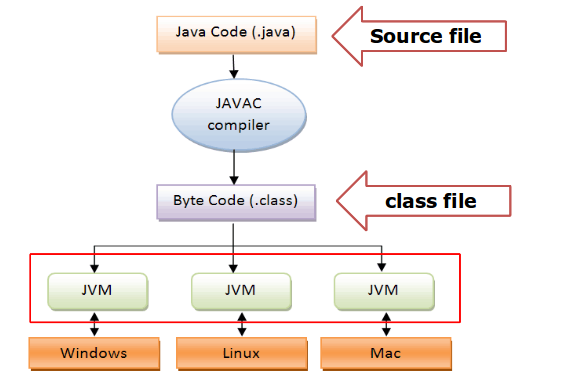
\includegraphics[scale=.4]{working-of-java-program.png}
 \end{center}
\end{figure}
\end{frame}

\begin{frame}{First Step Towards Programming}
 \textbf{JVM - Java Virtual Machine}
 \begin{itemize}
  \item When we compile a Java file, output is a \lstinline!.class file! but not an \textbf{.exe} file 
  \item \lstinline!.class! file consists of Java byte code which are understandable by JVM
  \item Java Virtual Machine interprets byte code into machine code depending upon the underlying operating system and hardware combination
  \item It is responsible for all the things like garbage collection, array bounds checking, etc...
 \end{itemize}
\end{frame}

\begin{frame}[fragile]{First Step Towards Programming}
 \textbf{Naming conventions}
 \begin{itemize}
  \item Package represents sub packages that contains group of classes and interfaces. Names of package in java are written lowercase letters
  \begin{verbatim}
java.lang   java.io   java.util
  \end{verbatim}
 \end{itemize}
\end{frame}

\begin{frame}[fragile]{First Step Towards Programming}
 \textbf{Naming conventions}
 \begin{itemize}
  \item Class is model for its objects. A class specifies properties and actions of objects. An interface is also similar to class. Each word of class name and interface name starts with a capital letter
  \begin{verbatim}
String DataInputStreamReader
  \end{verbatim}
 \end{itemize}
\end{frame}

\begin{frame}[fragile]{First Step Towards Programming}
 \begin{itemize}
  \item Class contain methods and variable. The first word of method name is in small letters; then from second word onwards, each new word should start with capital letter.
  
  \textbf{read()}, \textbf{getData()}, \textbf{viewEmployeeInfo()}
  
 \item Naming convention for variables names is same as that for methods
  
  \textbf{salary}, \textbf{empName}, \textbf{sumOfIntegers}
\end{itemize}
\end{frame}

\begin{frame}[fragile]{First Step Towards Programming}
\begin{itemize}

  \item Constants represents fixed values that can not be altered. Such constants can be written by using all capital letters
  
  \textbf{PI}
  \item All keywords should be written by using all small letters
  
  \textbf{public}, \textbf{static}, \textbf{class}, \textbf{int}
 \end{itemize}
\end{frame}

\begin{frame}[fragile]{First Step Towards Programming}
\begin{tabular}{p{9cm} r}
 Write a Java program to add four numbers. Rewrite above program by using two variables. & 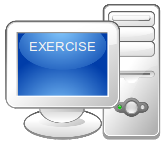
\includegraphics[scale=.3]{exercise.png} \\
 \end{tabular}
\end{frame}

\begin{frame}[fragile]{First Step Towards Programming}
\begin{block}{Solution}
\begin{lstlisting}
public class SumExample2 {
    public static void main(String[] args) {
        int next, sumSoFar;
        next = Integer.parseInt(args[0]);
        sumSoFar = next;
        next = Integer.parseInt(args[1]);
        sumSoFar += next;
        next = Integer.parseInt(args[2]);
        sumSoFar += next;
        next = Integer.parseInt(args[3]);
        sumSoFar += next;
        System.out.println("Sum: " + sumSoFar);
    }
}
 \end{lstlisting}
 \end{block}
\end{frame}

\begin{frame}[fragile]{First Step Towards Programming}
\begin{tabular}{p{8cm} r}
 Write a program to find the average of four numbers and then execute the program. & 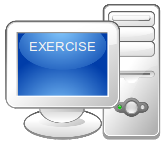
\includegraphics[scale=.4]{exercise.png} \\
 \end{tabular}
\end{frame}
\begin{frame}[fragile]{First Step Towards Programming}
\begin{block}{Solution} 
\begin{lstlisting}
public class AvgExample {
    public static void main(String[] args) {
        int next, sumSoFar;
        next = Integer.parseInt(args[0]);
        sumSoFar = next;
        next = Integer.parseInt(args[1]);
        sumSoFar += next;
        next = Integer.parseInt(args[2]);
        sumSoFar += next;
        next = Integer.parseInt(args[3]);
        sumSoFar += next;
        System.out.println("Average: " + sumSoFar / 4);
    }
}
 \end{lstlisting}
 \end{block}
\end{frame}

\begin{frame}{First Step Towards Programming}
\begin{figure}[H]
\begin{center}
 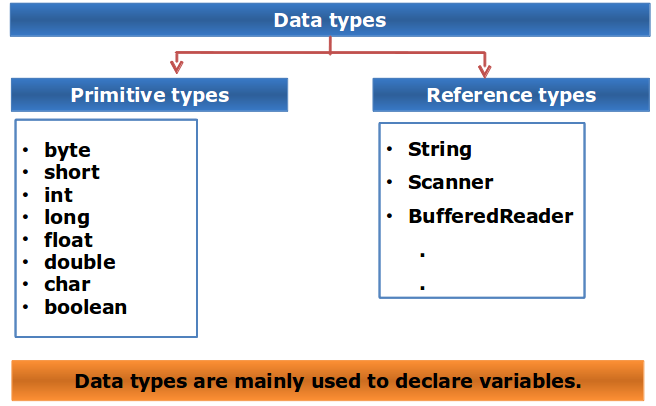
\includegraphics[scale=.3]{data-types.png}
\end{center}
\end{figure}
\end{frame}

\begin{frame}{First Step Towards Programming}
 \textbf{Variables}
 \small
 \begin{itemize}
  \item Basic unit of storage
  \item Stores the data at the address pointed by it
  \item Value and operation on it are determined by its datatype
 \end{itemize}
 \begin{figure}[H]
\begin{center}
 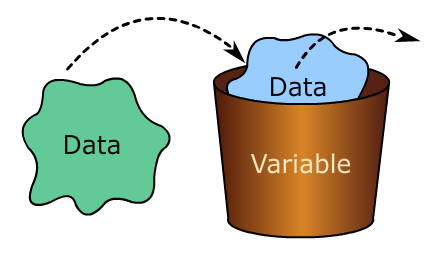
\includegraphics[scale=.15]{variables-storage.png}
\end{center}
\end{figure}
Variables are declared using primitive data types, such as \lstinline!byte, short, int, long, float, double, char, boolean,! etc.    
\end{frame}

\begin{frame}{First Step Towards Programming}
 \textbf{Variable - Naming Conventions }
 \begin{itemize}
  \item The name should convey the purpose of variable.
  \item All variable names must begin with an alphabet or with an underscore (\_) or with a dollar sign (\$) 
  
  \textbf{Good Practice:} Begin with a lowercase letter.
  \item No spaces or special characters are allowed
  \end{itemize}
\end{frame}

\begin{frame}{First Step Towards Programming}
  \begin{itemize}
  \item Can contain more than one word joined without spaces - may be with underscore.
 
 \textbf{Good Practice:} Use sentence case for each word except the first. 
  \item Java keywords (reserved words) are not allowed as variable names.
 
 \fbox{a, b, c, d, e... 
     
        name}
        
  \fbox{empName}
\end{itemize}
\end{frame}

\begin{frame}{First Step Towards Programming}
 \textbf{Variable - Declaration}
 
 The following is a way to declare a variable: 
 \begin{figure}[H]
\begin{center}
 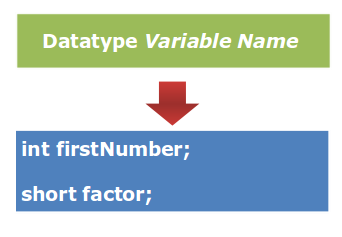
\includegraphics[scale=.4]{variable-declaration.png}
\end{center}
\end{figure} 
\end{frame}

\begin{frame}{First Step Towards Programming}
 \begin{figure}[H]
 \begin{center}
   
\includegraphics[scale=.5]{qa.png}   
 \end{center}
  \end{figure}
\end{frame}

\end{document}
